\chapter{利用掩食搜索双星中的星周盘} \label{chapter:form_evo}

\section{研究背景} \label{sec:diskbackground}

\subsection{星周盘简介} \label{sec:diskintro}

盘在天体物理中十分常见:从星系尺度的气体盘\cite{Binney1987,Gilmore1989}到致密星周围的吸积盘
\cite{Pringle1981},再小至行星形成的原行星盘(\S \ref{sec:pltfrmatntheory})以及形成卫星摇篮 --- 环
行星盘\cite{Smith1981,Latter2017,Mosqueira2003}。早在 17 世纪初盘,笛卡尔为了解释太阳系的行星
构型就引入了盘的概念,尽管那时候人类并未真正了解原恒星盘的模样\cite{Kawabe1993}。如今已迈入
中年的太阳系依然尚有黄道尘埃盘\cite{Dermott1994}、主小行星带以及库依柏带星子盘,这些也都是太
阳系纷乱的历史留下的残骸\cite{Dohnanyi1969}。


\begin{figure}[b]
\centering
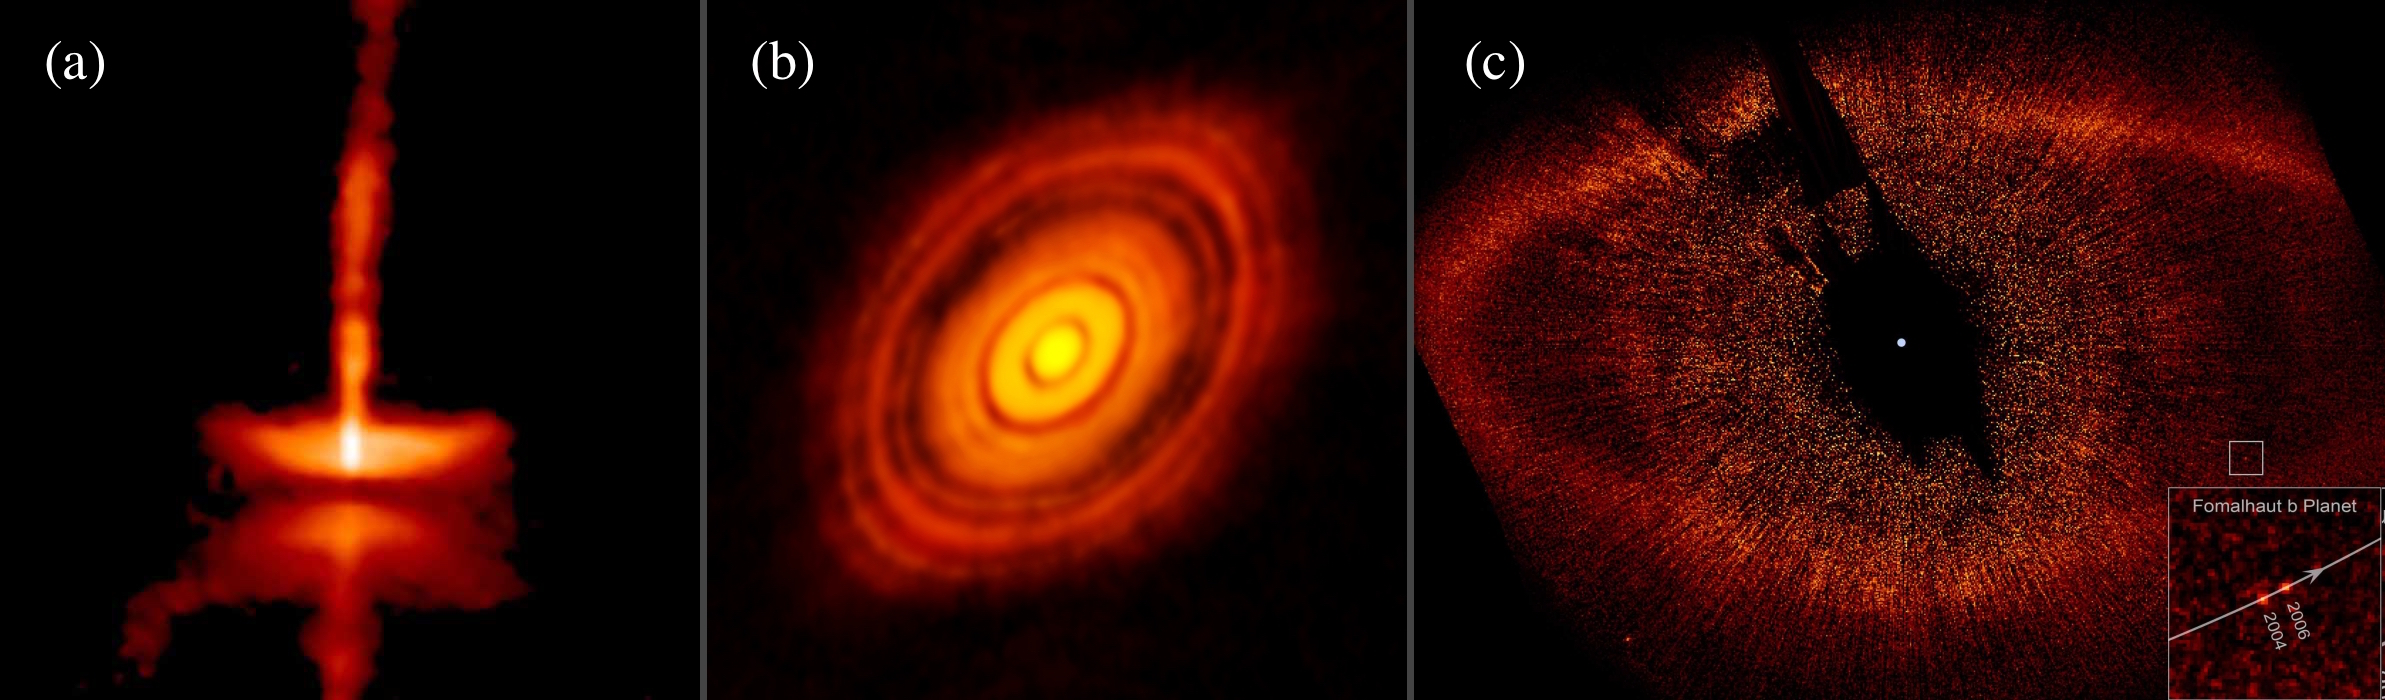
\includegraphics[width=1.0\textwidth]{figures/chapter3/f2_obsdisc.jpg}
\caption{原行星盘从早期、过渡到晚期三个不同的形态,其中 \textbf{(a)} HH 30 侧向视角的临变增厚盘,双极喷流清晰可见(版权:NASA, Alan Watson) \textbf{(b)} HL Tau (版权:ALMA - ESO/NAOJ/NRAO) \textbf{(c)} Formalhaut 残骸盘(版权:NASA,ESA 和 P. Kalas 等)。}
\label{fig:obsdisc}
\end{figure}

\begin{figure}[ht!]
\centering
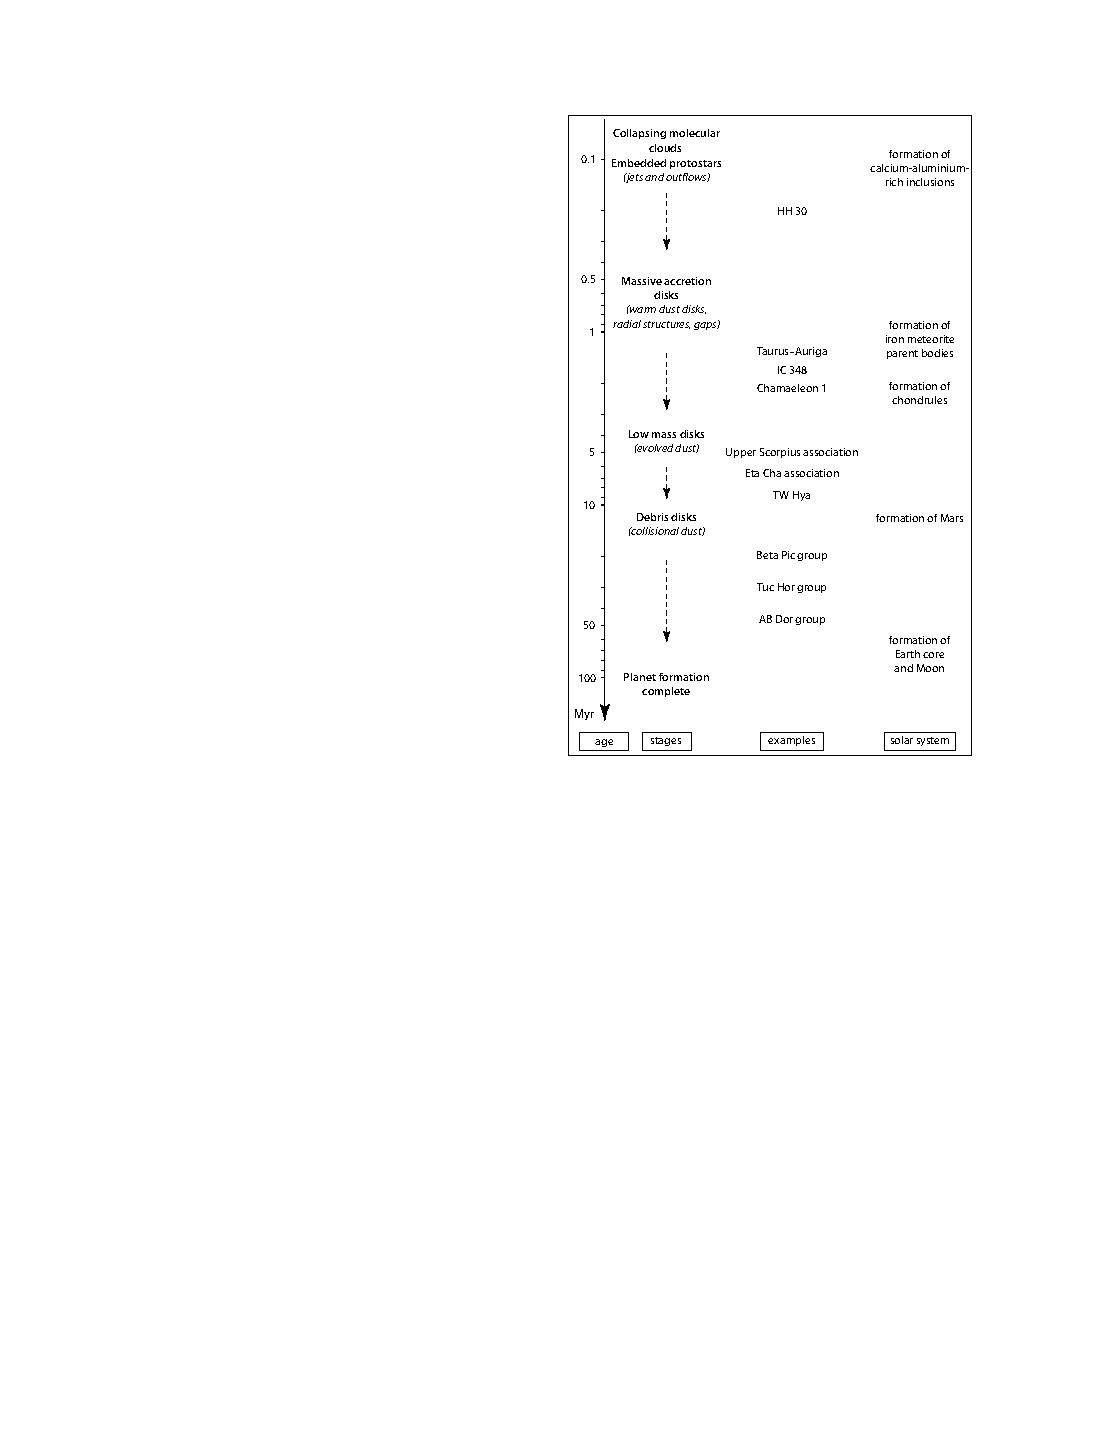
\includegraphics[scale=1.8]{figures/chapter3/f1_pfdisc.pdf}
\caption[行星形成的不同时期快照,从左至右分别为物理时间、形成阶段、系外行星系统实例与太阳系历史,版权所有人 Perryman。]{行星形成的不同时期快照,从左至右分别为时间、形成阶段、系外行星系统实例与太阳系历史。图片采取自书籍\citen{Perryman2014exohb},更详细的图请查看书籍\citen{ApaiLauretta2010}。}
\label{fig:pfdics}
\end{figure}


正如前文(参考\S \ref{sec:pltfrmatntheory})提到,行星孕育在星周盘内。此过程(如图 \ref{fig:obsdisc} 
与 \ref{fig:pfdics} 所示)包括早期分子云坍缩、恒星吸积盘内固体沉降、气体消散行星形成和最终演化为
残骸盘(Debris disk,又称碎屑盘)几个阶段。一般而言,描述气体的过程为内盘区域等离子磁层作用与
外层气体辐射转移两个过程\cite{Dullemond2010},而脱离气体耦合作用后的固体盘
一般则为 N 体引力作用(\S \ref{sec:clspftheory})。

星周盘(Circumstellar disk)观测到的辐射在理论上一般会用多黑体辐射谱来拟合。普朗克黑体谱
(Black body)有如下形式:

\begin{equation} \label{eq:blackbody}
\tif{B}_\nu (\tif{T}) = \frac{2h\nu^3}{c^2} \, \frac{1}{e^{h\nu / k\tif{T}}-1}
\end{equation} \myequation{黑体辐射}

\begin{figure}[t!]
\centering
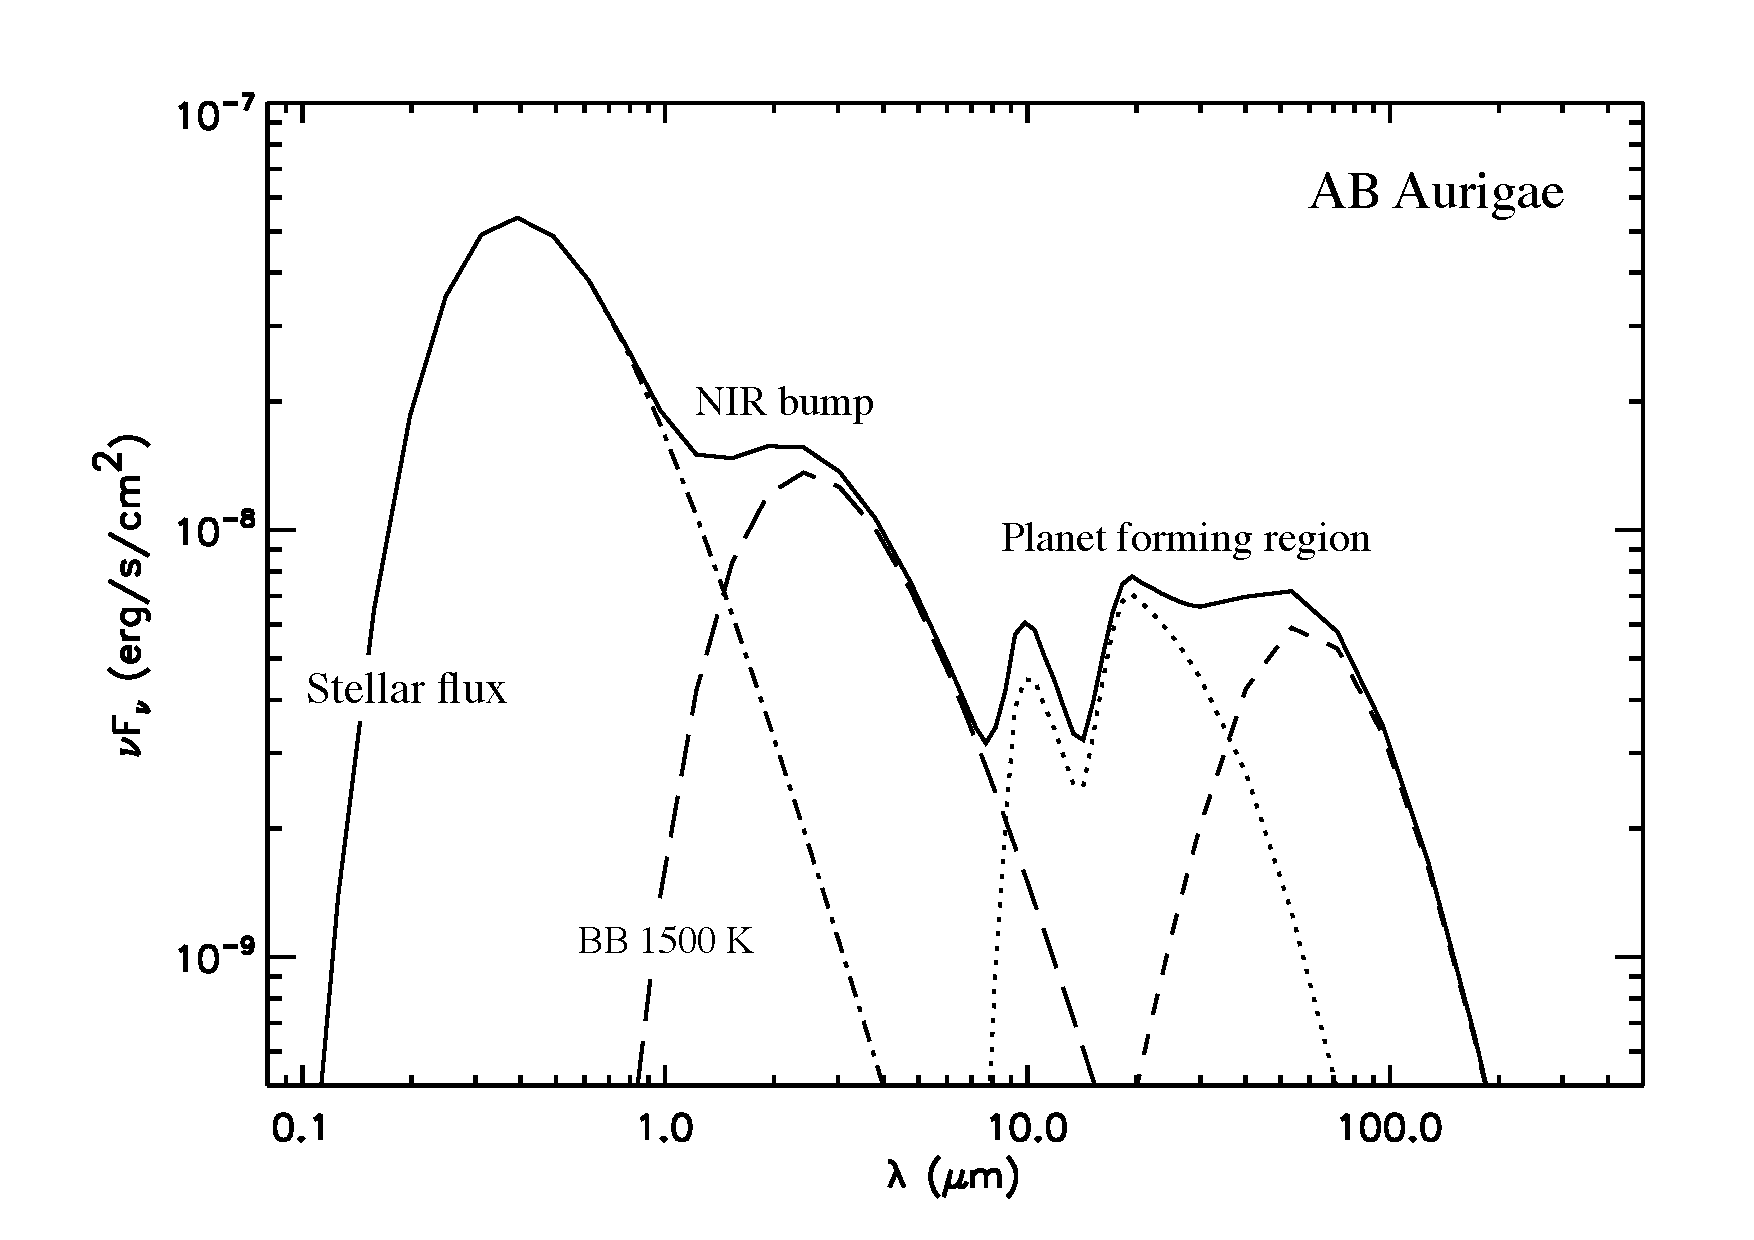
\includegraphics[width=1.0\textwidth]{figures/chapter3/f3_youngdisc.pdf}
\caption[AB Aurigae 系统理论谱能量分布图。从左至右分别表示恒星、有效温度为 1500 K 的星周内侧盘与外侧行星形成区域的黑体辐射组分。该图利用 Dullemond 开发的 CGPlus 程序制作。]{AB Aurigae 系统理论谱能量分布图。从左至右分别表示恒星、有效温度为 1500 K 的星周内侧盘与外侧行星形成区域的黑体辐射组分。此图利用 Dullemond 开发的 CGPlus 程序\footnotemark[1]制作。}
\label{fig:transdiscsed}
\end{figure}
\footnotetext{链接 \url{http://www.mpia.de/homes/dullemon/radtrans/fitcgplus/}。}

同样,径向对称且几何薄的星周盘总辐射可看作每个环状细盘黑体辐射的积分叠加,形式如下:

\begin{equation} \label{eq:diskrad}
\tif{F}_\nu = \frac{\cos \theta}{\tif{D}^2} \, \int \tif{B}_\nu (\tif{T}_\tif{d}) \, ( 1-e^{-\tau} ) \, 2\pi r \tif{d} r \ ,  
\end{equation} \myequation{多黑体盘总辐射量}
其中 $\theta$ 为观测者的视角,D 为观测者和源之间的距离。光深 $\tau$ 与盘内尘埃的不透明度
(Opacity)以及盘的面密度分布有关,因而上述公式所描述的星周盘谱能量分布(SED)函数是高度简并的函数。

%\begin{figure}[t]
%\centering
%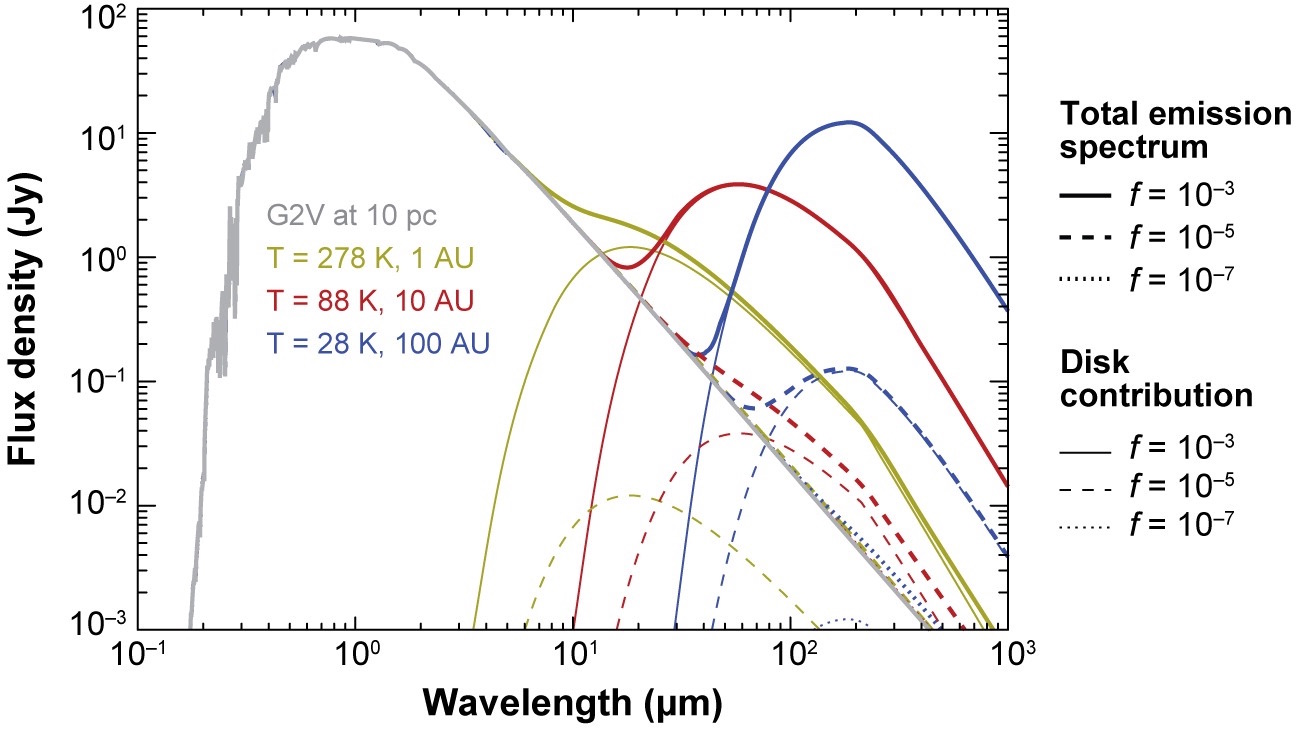
\includegraphics[width=1.0\textwidth]{figures/chapter3/f4_debrisdisc.jpg}
%\caption[类太阳(G2V)恒星于 10 pc 以外的理论辐射谱能量函数,长波范围的鼓包为星周残骸盘的黑体辐射。图片版权归 Wyatt 所有。]{类太阳(G2V)恒星于 10 pc 以外的理论辐射谱能量函数,长波范围的鼓包为星周残骸盘的黑体辐射。图片取自文献\citen{Wyatt2008}。}
%\label{fig:debrisdiscsed}
%\end{figure}


图 \ref{fig:transdiscsed} 为我们展示的为一个典型的原初恒星盘(Primordial disk)的能谱分布。此时从
内至外(波长由短至长),该 SED 主要包括四种成分:主星(9000 K)的黑体辐射,星周盘内侧区域
有效温度约 1500 K 的黑体辐射(近红外突起),行星形成区域(约从 1 AU 至 10 AU的尘埃连续谱)以
及最外侧亚毫米波段的盘最外侧。盘的演化是一个自内向外的消散过程,在观测中随着星周盘从原初恒
星盘演化至内侧区域最先被清空从而成为过渡盘(耗散相对快速,可被 ALMA 连续谱或成像观测
\cite{WilliamsCieza2011}),再最终演化成残骸盘(可被 HST 观测\cite{Wyatt2008})。需要说明的是,
由于星周盘的尘埃辐射主要集中在红外或更长的波段,所以观测中一般也将上述流量描述为红外光度比
例 $\tif{L}_\tif{IR}/\tif{L}_\tif{s}$。


\subsection{双星中星周盘研究背景} \label{sec:diskintro}

双星和多星系统在银河系中非常普遍,巡天显示类太阳恒星的成双概率大致为 45\%,并且其中约有 
10\% 为三星或更多星系统(文献 \citen{Duquennoy1991})。在双星系统形成早期,某一颗恒星可能会
拥有星周盘\cite{Bate1995},当观测者从远处观测时,会有一定的概率看到星周盘遮挡住此系统另外一
颗恒星。由于盘的尺度相比于恒星的尺度高出许多量级,因而一个随机取向的含盘系统可能会有非常高
的几何掩食概率\cite{Mamajek2012}。这样的掩食盘可以存在于行星形成中的双星系统(文献 
\citen{Galan2012})或卫星形成中的行星系统(文献 \citen{Mamajek2012})。掩食盘可以为我们提供非
常丰富的独到信息,如盘的不透明度以及三维立体结构(如土星环掩食,文献 \citen{Hedman2007})。

在观测上,$\epsilon$ Aurigae\cite{Guinan2002,Kloppenborg2010,Chadima2011} 与 EE Cephei 
\cite{Mikolajewski1999,Graczyk2003,Mikolajewski2005,Galan2012} 是两个相对熟知的盘状掩食双星系
统。最近 Mamajek 探测到太阳质量主序前恒星周围长时间、大深度的复杂盘掩食事件
\cite{Mamajek2012}。

在大麦云(Large Magellanic Cloud,下文简称 LMC)的掩食双星(EBs)中,Udalski 等人
\cite{Udalski2008,Graczyk2011}利用 OGLE-III 巡天发现了周期为 13.3 天的光变曲线中存在疑似盘结构
的系统 OGLE-LMC-ECL-17782,文献 \citen{Derekas2007} 曾认为此系统是不接食双星(Eclipsing 
Detached Binary,简称 ED)。在同一巡天计划样本中,拥有 468 天周期的系统 OGLE-LMC- 
ECL-11893 也被怀疑为掩食盘\cite{Dong2014}。下文,我们将利用 OGLE-III 巡天数据中 LMC 与 小麦
云(Small Magellanic Cloud,或简称 SMC)以及银盘(Galactic Disc,下文统称 GD)观测到的 EB 样
本\cite{Graczyk2011,Pawlak2013,Pietrukowicz2013} 光变曲线中分析额外可能的掩食盘事件。

近年来,对太阳附近恒星以及恒星形成区的红外以及毫米波段巡天显示恒星的年龄、质量以及伴星的存
在会影响恒星周围是否存在可探测的盘状结构
\cite{Haisch2001,Bouwman2006,Hernandez2007,Harris2012,DeRosa2013}。在对 OGLE-III EB 的研究
显示 EB 系统在大型巡天中是一个近乎确定、完备的样本
\cite{Graczyk2011,Pawlak2013,Pietrukowicz2013}。另外,我们还将本文 LMC  EB 掩食盘的搜寻概率与
近年已有的银河系红外(毫米波)的盘探测率做了对比。这种另辟蹊径的做法也可能为今后搜寻活动提
供新的导向。

\section{利用双星掩食光变曲线搜索星周盘} \label{sec:discsineb}

文献 \citen{Graczyk2010} 提到利用光变曲线中星等分布(或者统计矩阵)可以区分不同的变星以
及 EBs。根据他们的方案,我们在 EBs 的光变曲线的在食区间使用同样的方法,目标是将以往 EB 系统
中可能的掩食盘结构区分并探测出。在 EBs 中,其中一颗掩食另外一颗星通常会造成一个三角、方形或
者高斯轮廓的掩食光变曲线。在本文,我们则利用光变曲线中和这些普通情况不同的掩食形状来区分可
能的掩食盘系统。这些结构包括不对称型(EE Cep 或 J1407,文献 
\citen{Galan2012,Mamajek2012}),W-型掩食形状($\epsilon$ Aurigae,文献 \citen{Guinan2002} )
或者宽平台型(如 OGLE-LMC- ECL-17782,文献 \citen{Graczyk2011})。如果我们探测到此类特殊结
构,我们则会将该系统标注为掩食盘候选体,尽管我们并未真正看到盘本身的旋转结构。


\subsection{搜索掩食盘的方法} \label{sec:discebmeth}

下面我们将简要介绍搜索掩食盘的过程,该过程不仅可以利用于 OGLE-III LMC,SMC 和 GD 的 EB 样
本,也可以推广至任何其他的巡天中。

\begin{enumerate}
\item 提取 OGLE-III 巡天中被识别成 ED 系统的相位叠加光变曲线,并计算该曲线的平均星等值与掩食
外光变曲线平台的弥散值;
\item 抛弃信噪比太低、观测点数太少或光变曲线平台部分弥散值太大(暗示此源可能为变星)的系统;
\item 利用程序自动识别主掩食和次掩食以及它们彼此互掩开始(初亏)和结束(复圆)的位置,这样便
可确定光变曲线掩食内的窗口;
\item 计算掩食内光变曲线的斜度(Skewness)与峰度(Kurtosis)以及星等的分布统计值。
\end{enumerate}

我们并没有考虑低信噪比、观测点太少的光变曲线,因为此类系统的在食部分并不能被有效地识别出。
这部分系统的斜度和峰度参数不能被很好的反演,从而造成成倍的额外掩食盘「假阳性」候选体。而如
何计算这些 EBs 系统掩食外的星等标准差以及识别进食(ingress)和出食(egress)粗略介绍如下:


\begin{enumerate}
\item 首先,我们将 OGLE-III 巡天计划中的 LMC,SMC 和 GD 得到的 EDs 光变曲线在它们各自的轨
道周期\cite{Graczyk2011,Pawlak2013,Pietrukowicz2013}上做折叠;

\item 接下来计算整条光变曲线(掩食内以及掩食外)的中值(median value),并记作 $\mu_\tif{L}$。
因为这边取的是中值,从而此值应大约为 EB 光变曲线掩食外的平均星等;

\item 然后对整条光变曲线做宽度为五个点的点滑动平均(box smoothing),将最暗(星等值最大)的
点标记为主掩食甚(伴星遮挡主星面积最大的时刻),用 $\theta_\tif{p}$ 表示。而次掩食甚时刻 $
\theta_\tif{s}$ 则定义为在 $\theta_i$ 处,$|m(\theta_i) - m(\theta_\tif{m})|$ 达到最大值,其中 $
\theta_\tif{m}$ 等于 $(\theta_i+ \theta_\tif{p})/2$,而 $m(\theta)$ 为相位 $\theta$ 处的星等值;

\item 选取在 $[\theta_\tif{m} - 0.05, \, \theta_\tif{m} + 0.05]$ (也即绝对相位宽度为 0.1)区间内计算这
段光变曲线的标准差:$\sigma_\tif{L}$,也即掩食外光变曲线的弥散度;

\item 而光变曲线的主掩部分则定义为星等值比平均值低 $1\sigma$,即 $m > \mu_\tif{L} + \sigma_\tif{L}
$ 并且区间内包含 $\theta_\tif{p}$. 同样的方法也可以定义包含 $\theta_\tif{s}$ 的次掩食部分。

\item 最后将上步得到的两段主次掩食内的光变曲线从整条光变曲线中扣除,并重新计算第 2 步中的中值
以及弥散。这样做可以得到更加真实的光变曲线掩食外部分。利用新得到的 $\mu_\tif{L}$ 和 $\sigma_
\tif{L}$,我们可以在再次回到上一步划分主次掩内的光变曲线。值得注意的是这里得到的 $\mu_\tif{L}$ 
和 $\sigma_\tif{L}$ 两者之值将被用来计算掩食内光变曲线的斜度和峰度。
\end{enumerate}

\begin{figure}[ht!]
\centering
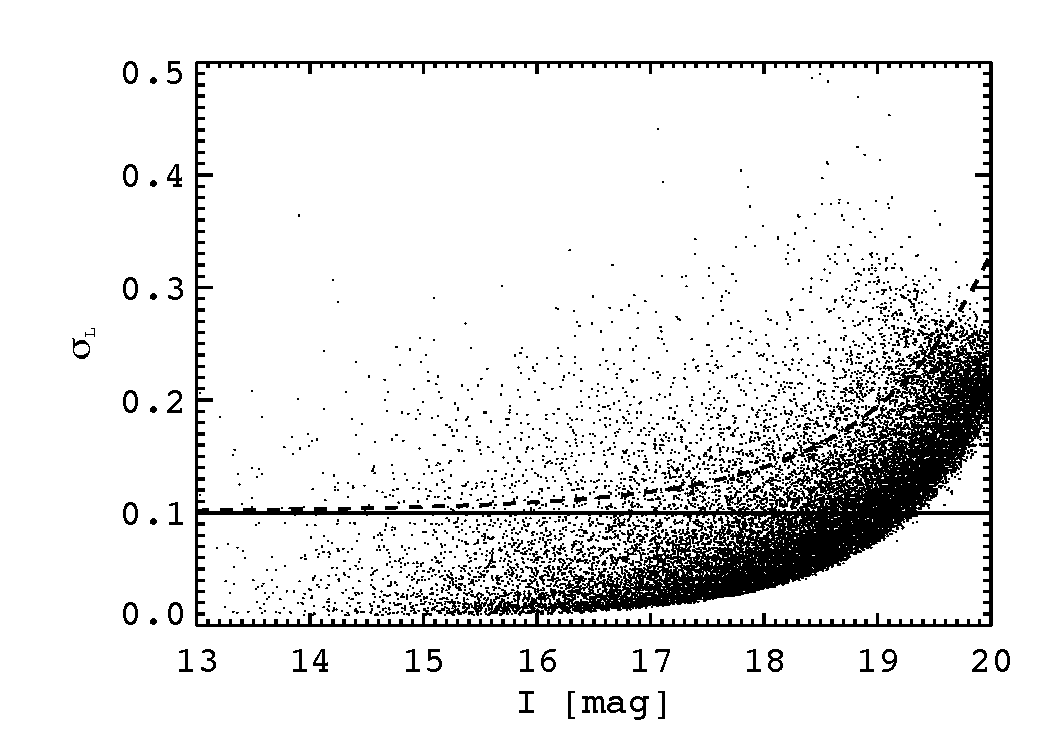
\includegraphics[width=1.0\textwidth,trim={0.4in 0.2in 0 0}]{figures/chapter3/f4_magerr.pdf}
\caption{OGLE-III LMC EBs 样本 $i$ 波段星等与该波段掩食外的星等标准偏差散点图。为了着重显示高信噪比的系统,我们人为去除了 $i$ 波段星等大于 19.3 的 EBs。另外实线上侧的掩食外星等弥散度 $\sigma_\tif{L} > 0.1$ 也被舍去。另外,虚线表示 $\sigma_\tif{L} > \sigma_\tif{c} + 0.1 $,其中 $\sigma_\tif{c}$ 为极限星等误差。我们也尝试过该选择判据,结果显示两种方法并不能影响图 \ref{fig:lmcks} 中的实线方框内的点。}
\label{fig:magerr}
\end{figure}

下面我们将以 OGLE-III LMC 内共 26,121 个 EB 样本\cite{Graczyk2011}为例,介绍如何得到可靠的斜度
和峰度。图 \ref{fig:magerr} 为对该样本计算得到的 $\sigma_\tif{L}$ 与 $i$ 波段星等的分布函数图。从图
中可以明显看到信噪比较差的系统总是暗源,这也很自然,因为测光误差总是依赖于星等。为了避免用来
搜寻掩食盘的样本性噪比太低,我们将 $i$ 波段测光星等大于 19.3 以及弥散大于 0.1 的系统从样本中剔
除。

另外,如果掩食窗口内的观测点数太少,我们也同样不能精确的计算星等分布的多极矩。如果在掩食窗口
内光变曲线的点数为 $N_\tif{ecl}$,那么 $N_\tif{ecl}/N \le 0.25$ 的系统也会被排除在外,其中 $N$ 为整
个光变曲线的观测点数。此选择条件还可以将我们的样本限制为 EDs。而且为了保证斜度和峰度计算值
的可靠度,只有 $N_\tif{ecl} > 20$ 的系统才会被留下来用作下一步的计算。最后,我们还将分析的系统
限制在较深的掩食中。为了寻找主掩食盘(即伴星的星周盘),我们的分析中只留下光变曲线主掩深度 $|
m(\theta_\tif{p}) - \mu_\tif{L}| > 4 \sigma_\tif{L}$ 的系统,其中 $|m(\theta_\tif{p})  - \mu_\tif{L}|$ 用来衡量
主掩食深度。同样次掩食盘(主星的星周盘)判据则定为 $|m(\theta_\tif{s}) - \mu_\tif{L}| > 3 \sigma_
\tif{L}$。之所以这样选取是因为当以上两个判据变得不那么严格时,最后的结果中会包含相当多的污染源
以至于掩食盘候选体被淹没在其他系统中,这些系统并没有掩食盘而只是星等分布接近掩食盘系统。

在主掩和次掩食内,星等分布的斜度 S 以及峰度 K 的计算公式如下:

\begin{equation} \label{eq:skew}
S =  \frac{1}{N} \sum_{i=0}^{N-1} \left(\frac{m_i - \mu}{\sigma_\tif{L}}\right)^3 
\end{equation}  \myequation{样本高阶矩 --- 斜度的计算公式}
\begin{equation} \label{eq:kur}
K =  \frac{1}{N} \sum_{i=0}^{N-1} \left(\frac{m_i - \mu}{\sigma_\tif{L}}\right)^4 - 3 \, \ , 
\end{equation} \myequation{样本高阶矩 --- 峰度的计算公式}
其中掩食窗口内的星等平均值 $\mu = \frac{1}{N} \sum_{i=0}^{N-1} m_i$。需要留意的是这边的平均星等 
$\mu$ 和前一小节的中值 $\mu_\tif{L}$ 不能混为一谈。$N$ 为掩食窗口内折叠后光变曲线的观测点数
目,而 $m_i$ 则是它们中每一个观测点的星等值。


\begin{figure}[t]
\centering
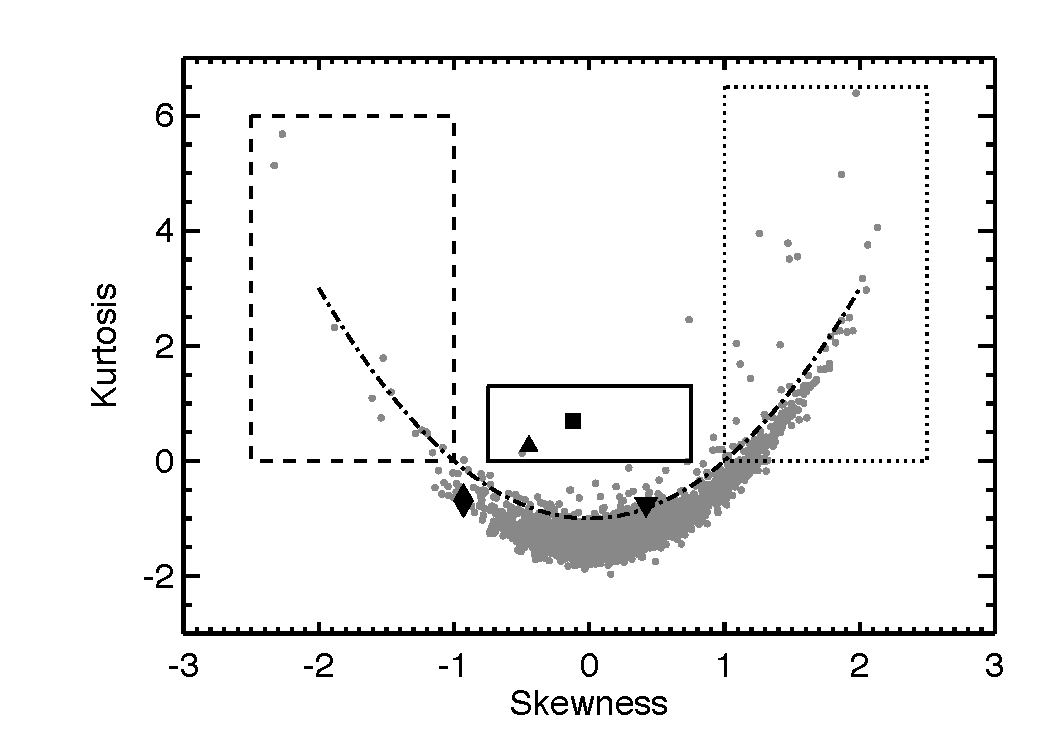
\includegraphics[width=1.0\textwidth,trim={0.4in 0.2in 0 0}]{figures/chapter3/f5_lmcks.pdf}
\caption{由 LMC 中 2823 个低噪声 EBs 样本计算得到的主掩食内斜度和峰度分布图。OGLE-LMC-ECL-17782 和 OGLE-LMC-ECL-11893 分别用实心方块与三角形标注。为了区分不同性质的系统,我们将该图划分为四个不同的区域:虚线、实线、点线以及点虚线,它们分别代表着拥有不同掩食内光变曲线形状的 EBs --- 实线区域内为掩食盘的候选体,而点虚线(近似 $K=S^2-1$ 抛物线)则为星等分布的整体形状。EE Cep 和 $\epsilon$ Aur 也分别用倒三角与菱形标注,可以看到斜度峰度方法并不能很好的区分 EE Cep 和 $\epsilon$ Aur 和其他 EBs。}
\label{fig:lmcks}
\end{figure}


\subsection{掩食窗口内星等分布} \label{sec:discebresult}

我们首先尝试将上述方法运用到 OGLE-III 巡天中 LMC EBs 的样本\cite{Graczyk2011}。OGLE-III 巡天在
凝视 LMC 的视场大约有 40 平方度的大小,视场内也探测到近 320 万个源\cite{Ulaczyk2012}。其中 
26,121 个源被证认为 EBs\cite{Graczyk2011}。为了从大量数据中搜索这些双星,Graczyk 和 Eyer 将 $i$ 
波段的星等限制在 20 以内,至少拥有 120 个测光点,并且周期限定在 $1.0015 < P< 475$ 天
\cite{Graczyk2010},他们搜索这些双星的周期运用了 Stellingwerf 提出的 phase dispersion minimization 
方法\cite{Stellingwerf1978}。

上一小节提到选取限定条件,于是我们从 LMC 26,121 个系统中挑选出了 2823 个高测光连续度且测光精
度较好的 EB 系统,这些系统被成为高信噪比 LMC EBs。计算出这些高信噪比 LMC EBs 的斜度以及峰
度后(图 \ref{fig:lmcks} 中),之前两个已发现的掩食盘系统 OGLE-LMC-ECL-17782 和 OGLE-LMC-
ECL-11893 落在了实线方框区域($|S| < 1.0$,$K > 0$)。同样,我们定了双曲线 $K = S^2 - 1$(以指
代普通 EBs)来区分主掩和次掩食内是否明显有平台期。这里明显的判断标准则落在了 $S = 0$ 和 $K = 
0$ 附近。类似的对于系统 EE Cep 与  $\epsilon$ Aur,我们采用了 Galan 等人\cite{Galan2012}观测到的 
V 波段掩食数据\footnote{\url{http://vizier.cfa.harvard.edu/viz-bin/VizieR?-source=J/A+A/544/A53}}和 
Parthasarathy 于 1982 至 1988 年之间\cite{Parthasarathy1986}观测的 V 波段数据\footnote{\url{http://
www.hposoft.com/campaign09.html}} 来计算斜度和峰度,然而他们并没有很好的和其他系统分离开。

那么究竟什么原因导致上述 OGLE-LMC-ECL-17782 和 OGLE-LMC-ECL-11893 两个系统在斜度 --- 峰度
分布图中明显突出呢?从方程 \ref{eq:skew} 和 \ref{eq:kur} 出发,在统计中峰度可以用来指示星等分布的
集中度,而斜度则用可类比为星等分布的不对称度(即星等峰值在其平均值的明或暗两端)。正是如此,
我们才将图 \ref{fig:lmcks} 划分成四个区域:实线、点线、虚线和其余区域。点线区域内 EBs 掩食内星等
的分布集中在进出掩食附近,因此拥有正斜度(例如系统 OGLE-LMC-ECL-02192,参考图 
\ref{fig:lmc02192})。而虚线方框内 EBs 则因拥有方形平台底部贯穿最大掩食(食甚)而正好拥有相符号
反的斜度(例如系统 OGLE-LMC-ECL-12966,参考图 \ref{fig:lmc12966})。

\begin{figure}[t]
\centering
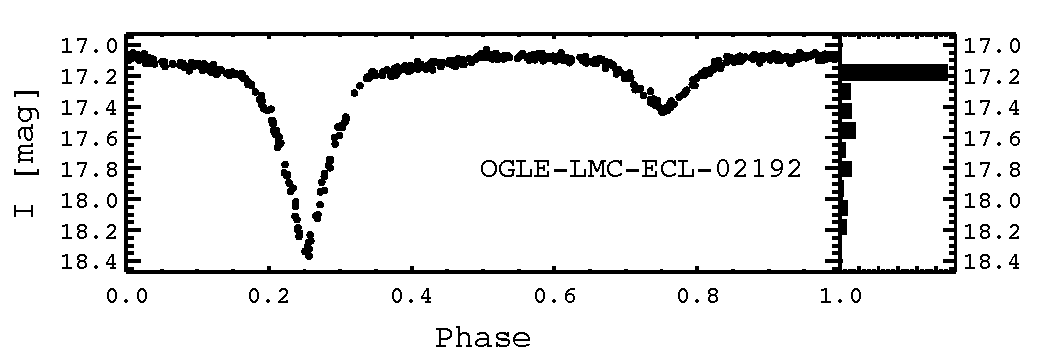
\includegraphics[width=0.98\textwidth,trim={0.0in 0.2in 0 0}]{figures/chapter3/f6_lmc02192.pdf}
\caption{OGLE-LMC-ECL-02192 的周期($P = 1.59\, \tif{d}$)叠加光变曲线(左侧),该系统属于 ED,并且其中一颗恒星的洛希瓣被充满。右栏为掩食内星等分布柱状图,入食与出食相位分别为 0.1 和 0.5。该系统入出掩食较缓慢,星等分布拥有明亮尾巴,因而拥有正斜度($S=1.94$,$K=4.98$),在图 \ref{fig:lmcks} 中处于点线方框内。}
\label{fig:lmc02192}
\end{figure}

如果系统中拥有可能的掩食盘候选体,那么光变曲线中掩食内的星等统计分布则与上述两种情况完全不
同。通常而言这样的系统会在光变曲线侧翼中(掩食半遮掩状态)包含平台状的结构。这也并不难理解,
因为盘的几何尺度往往比恒星尺度大,在伴星掩食主星之前,伴星周围的盘会先开始掩食。如果盘的结构
不复杂(多环、倾斜或单边状),那么在恒星掩食开始前会有一段盘掩食的平坦光变区间,这也正是系统 
OGLE-LMC-ECL-11893(图 \ref{fig:lmc11893})和 OGLE-LMC-ECL-17782(图 \ref{fig:lmc11782})与
图 \ref{fig:lmcks} 中其他 EBs 的不同之处。

\begin{figure}[t]
\centering
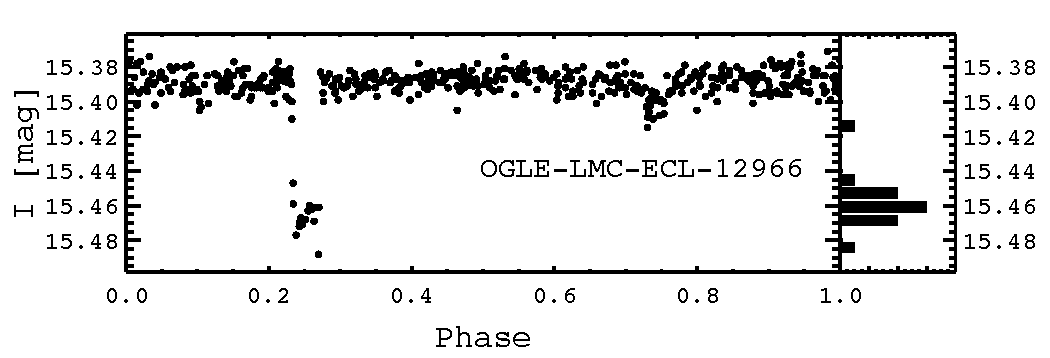
\includegraphics[width=0.98\textwidth,trim={0.0in 0.2in 0 0}]{figures/chapter3/f7_lmc12966.pdf}
\caption{与图 \ref{fig:lmc02192} 相同,但为系统 OGLE-LMC-ECL-12966($P = 239.6\, \tif{d}$)。该系统同样为 ED,但不同的是由于掩食内光变曲线呈方波形状,从而右侧星等分布集中在暗端,斜度也因此为负值($S=-1.35$,$K=1.21$)。在图 \ref{fig:lmcks} 中位于虚线框内。}
\label{fig:lmc12966}
\end{figure}


\begin{figure}[ht!]
\centering
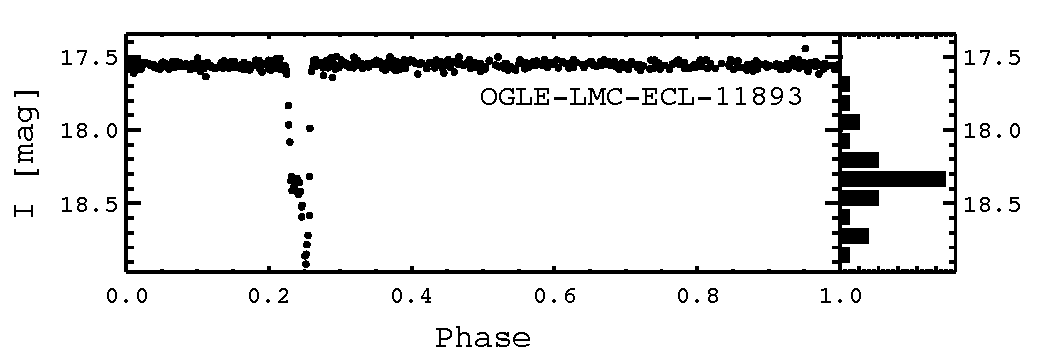
\includegraphics[width=0.98\textwidth,trim={0.0in 0.2in 0 0}]{figures/chapter3/f8_lmc11893.pdf}
\caption{与图 \ref{fig:lmc02192} 相同,但为系统 OGLE-LMC-ECL-11893($P = 468.045\, \tif{d}$)。该系的星等分布拥有斜度接近于零和正峰度($S=-0.45$,$K=0.25$),这是因为掩食内中央区域有一段平台期,在图 \ref{fig:lmcks} 中位于实线框内。}
\label{fig:lmc11893}
\end{figure}


\begin{figure}[ht!]
\centering
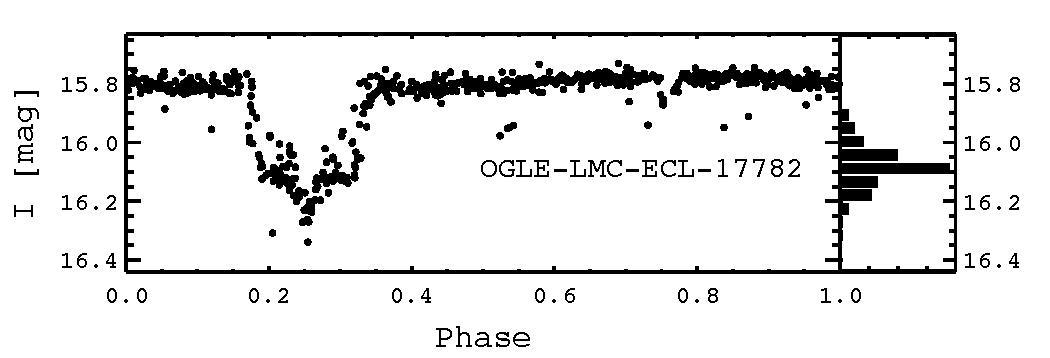
\includegraphics[width=0.98\textwidth,trim={0.0in 0.2in 0 0}]{figures/chapter3/f9_lmc11782.pdf}
\caption[与图 \ref{fig:lmc02192} 相同,但为系统 OGLE-LMC-ECL-17782($P=13.353\,\tif{d}$)。此系统为前人已识别的掩食盘候选体。由于该系统的掩食内星等分布同样拥有平台阶段,因而斜度与峰度值接近系统 OGLE LMC-ECL-11893($S=0.12$,$K=0.89$)。可以从图中看到该系统拥有变化的掩食轮廓和深度。]{与图 \ref{fig:lmc02192} 相同,但为系统 OGLE-LMC-ECL-17782($P=13.353\,\tif{d}$)。此系统为前人已识别的掩食盘候选体\cite{Graczyk2011}。由于该系统的掩食内星等分布同样拥有平台阶段,因而斜度与峰度值接近系统 OGLE LMC-ECL-11893($S=0.12$,$K=0.89$)。可以从图中看到该系统拥有变化的掩食轮廓和深度。}
\label{fig:lmc11782}
\end{figure}


需要说明的是,峰度斜度的筛选法并不能区分出以往类似 EE Cep 的进出掩食不对称结构,同样对诸如$
\epsilon$ Aur 的“W 型”掩食结构也没办法分离与识别,因为峰度斜度只能用来描述掩食内观测点的不均匀
性。从图 \ref{fig:lmcks} 中,还有另外一个系统 OGLE-LMC-ECL-17138 也在前面提到的实线方框(即掩
食盘可能区域)内。该系统的光变曲线以及掩食内星等统计如图 \ref{fig:lmc17138},似乎该系统并未显示
盘状掩食结构,那么为什么它的统计多极矩计算值和两个候选体类似呢?这里,我们将此峰度归结于这颗
系统存在掩食深度变化(Eclipsing Depth Variation,简称 EDV)。当我们在该系统单个周期内检查光变
曲线时,发现它的掩食内是明显的方波形状(峰度较小)。然而在周期折叠后的光变图中,该系统不同掩
食深度叠加后的确会成为该方法的例外,因而我们通过眼睛查看确认后将该系统排除出掩食盘候选体。

\begin{figure}[t]
\centering
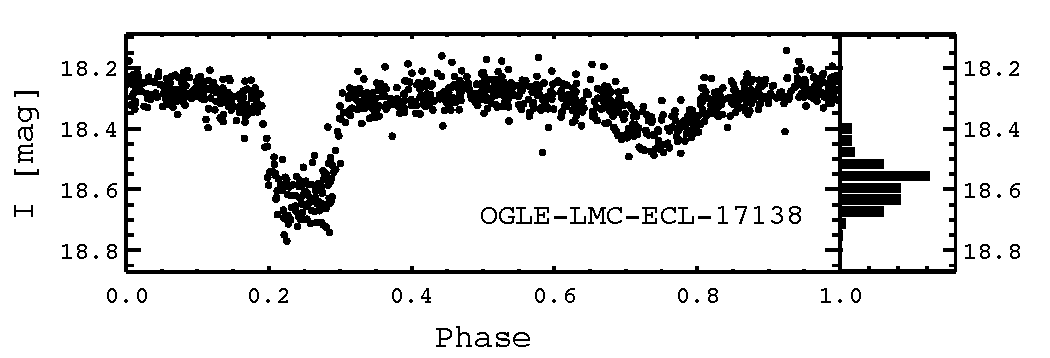
\includegraphics[width=0.98\textwidth,trim={0.0in 0.2in 0 0}]{figures/chapter3/f10_lmc17138.pdf}
\caption{与图 \ref{fig:lmc02192} 相同,但为系统OGLE LMC-ECL-17138($P = 11.1 \tif{d}$)。它是在 图 \ref{fig:lmcks} 实线框中的唯一的污染源。此系统拥有与掩食盘候选体 OGLE-LMC-ECL-11893 与 OGLE-LMC-ECL-17782 类似的掩食内星等分布斜度与峰度统计值($S=-0.36$ and $K=-0.02$),这是由系统的掩食深度变化所导致的。}
\label{fig:lmc17138}
\end{figure}


接下来,我们将该方法流程应用到 OGLE-III LMC EBs 次掩食,SMC EBs 主、次掩食以及 GD EBs 样本
中。在 LMC EBs 样本中,我们运用同样的方法总共找到 418 个高信噪比次掩食系统,然而在这些系统中
并没有找到掩食盘的候选体。而对与 SMC 中 EBs 样本,我们将 6,138 个系统缩小至 748 个高信噪比主
掩食,同样计算出斜度和峰度分布图并分析后我们得到了一个疑似掩食盘系统 OGLE- SMC-ECL-0007,
由于该双星周期为 $1.211 \tif{d}$ 并且主次掩食都发现了同样的非对称结构,因此猜测两颗星同时拥有掩
食盘的概率应该不会大。与此同时,文献 \citen{Pawlak2013} 的研究显示该系统为视线方向上的前景晚型
恒星,单独查看周期发现光变曲线在掩食内仅拥有 3---4 个测光点,因此我们怀疑该双星有 ETV 或者存在
星风,但也并不能对该系统下定论。

\begin{figure}[t]
\centering
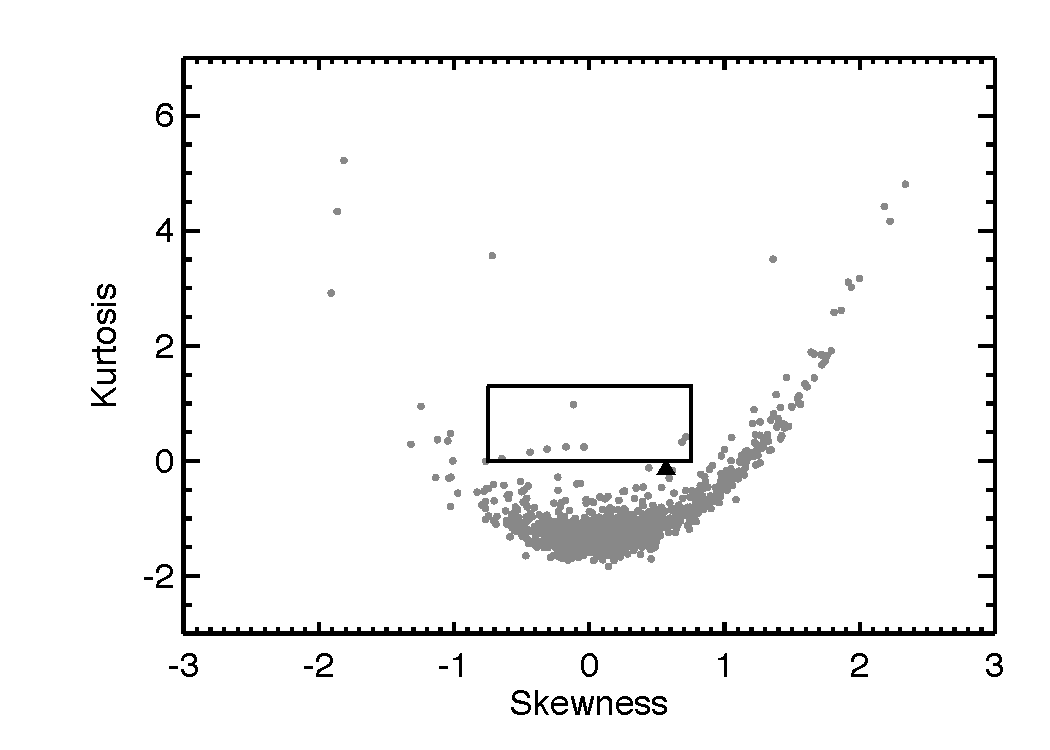
\includegraphics[width=0.98\textwidth,trim={0.4in 0.2in 0 0}]{figures/chapter3/f11_smcks.pdf}
\caption{与图 \ref{fig:lmcks} 相同,此图样本为 SMC EBs。我们同样检验了掩食盘在斜度峰度图上的可能区域,发现所有的点几乎都没有任何掩食盘的迹象,除了用三角形标注的系统 OGLE-SMC-ECL-0007(参见图 \ref{fig:smc0007})。虽然该系统在实线方框之外,光变曲线掩食内部分有些微的不对称性。}
\label{fig:smcks}
\end{figure}


\begin{figure}[t]
\centering
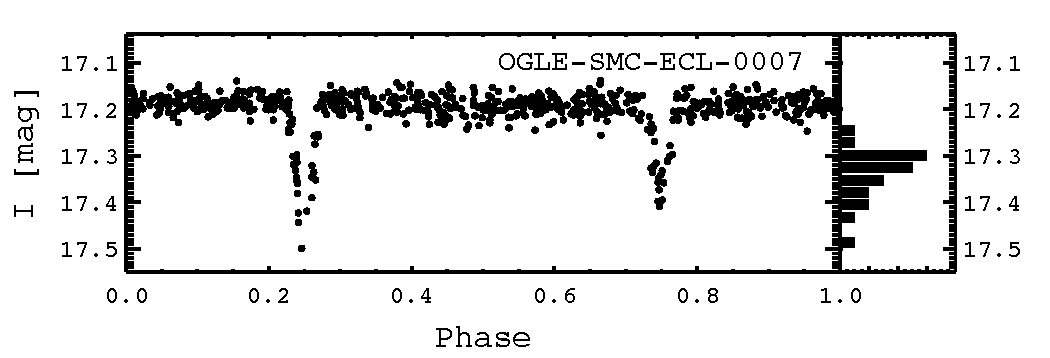
\includegraphics[width=0.98\textwidth,trim={0.0in 0.2in 0 0}]{figures/chapter3/f12_smc0007.pdf}
\caption{与图 \ref{fig:lmc02192} 相同,但为系统 OGLE-SMC-ECL-0007($P = 1.211 \tif{d}$)。此系统为 SMC EBs 中可能的掩食盘例子。它掩食内星等分布统计显示出不对成性$S=0.57$ and $K=-0.15$)。可以看出来主掩和次掩都为不对称结构,应为该系统为短周期双星,因此我们怀疑它同样存在 ETV。}
\label{fig:smc0007}
\end{figure}

最后,前文提到的方法被应用到 GD EBs 样本中,同样未发现明显的掩食盘信号(共 570 个高信噪比系
统)。这可能是因为 GD 样本的掩食深度噪声比相对于 LMC 甚至 SMC 都要差一些,并且在 GD 样本中
大部分恒星都偏年老,而盘的年龄要远远小于恒星的年龄。需要说明的是,在 GD EBs 样本中,最长周期
仅为 $P = 103.502 $天,在掩食盘搜索工作中,双星的间距越大,那么它们周围盘的洛希半径也就越
大,充满洛希半径的盘也更容易被巡天发现(关于洛希瓣请参考附录图 \ref{fig:rocher}。)。

\subsection{LMC 中掩食盘候选体的性质} \label{sec:discebprop}

文献 \cite{Derekas2007,Graczyk2011} 中提到 LMC 中 EBs 的色指数星等分布图具有双峰结构,分别为偏蓝
的近主序星和偏红的红巨星、超巨星(参见 \S \ref{apdx:HRdiagram},图 \ref{fig:hrdiagram})。那么在 
OGLE-III 的 EBs 中有多少为主序星呢?如果在这里我们定义$V - I \le 0.5 $ mag 为主序,那么在这 2823 
个高信噪比的 LMC EBs 中,一共有 2,471 对在主序附近。


我们将所有高信噪比 LMC EBs 的色指数 --- 星等画在图 \ref{fig:lmctracks} 中,可以看到 OGLE-LMC-ECL- 
17782(实心方框)和 OGLE-LMC-ECL-11893(实心三角)拥有接近与主序性质。此图采用文献 
\citen{Marigo2008} 提供的 Pandova internet server\footnote{\url{http://stev.oapd.inaf.it/cgi-bin/cmd}} 来制作
金属丰度为 $Z=0.006$(LMC 的经典丰度值)年龄跨越 $\log_{10}$(age/yr)$=6.0-9.0$ 且步长为 $\Delta 
\log_{10}$(age)$=0.1$ 的颜色---星等图。图中我们保留原始的 LMC EB 样本的星等与色指数值不变,而是将等年
龄线做了消光红移修正。修正量为 $A_V=0.55$(文献\citen{Zaritsky2004}),距离模数为 $\delta m=18.48$ mag 
(\citen{Walker2012})。下面我们将详细分析这两个系统。


\begin{figure}[t]
\centering
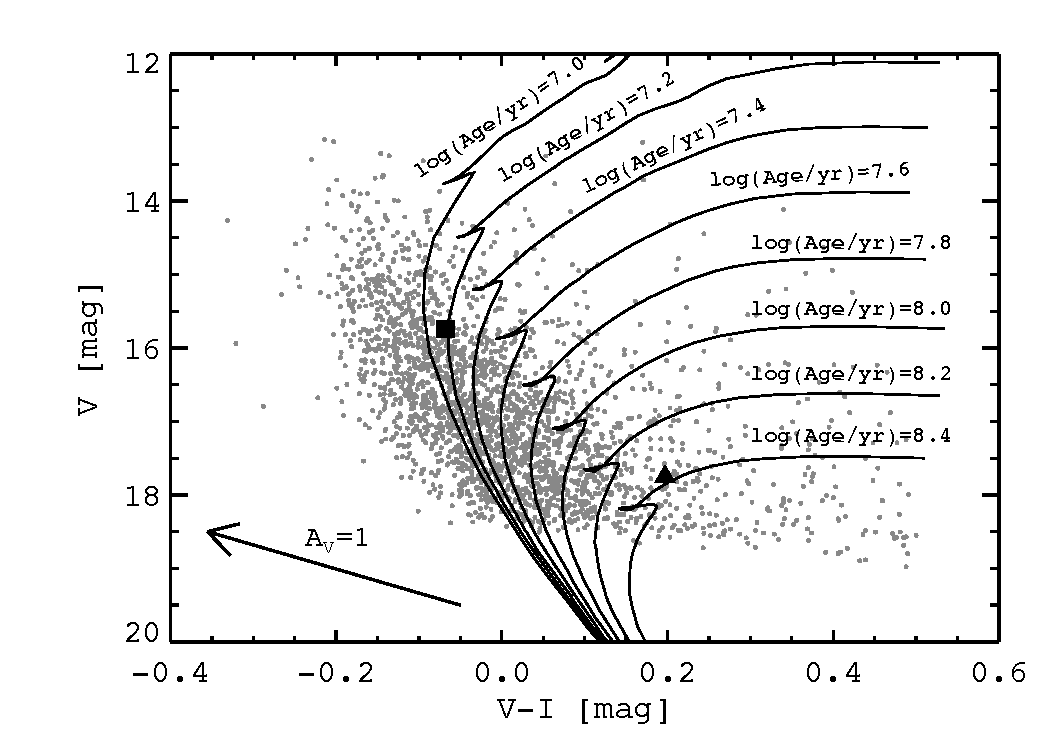
\includegraphics[width=1.0\textwidth]{figures/chapter3/f13_isotracks.pdf}
\caption[ LMC 低噪声 EB 样本的颜色 --- 星等分布图,其中 $V - I \le 0.5 $ mag 定义为主序系统。那么前文提到的掩食盘候选系统 OGLE-LMC-ECL- 17782(实心方框)和 OGLE-LMC-ECL-11893(实心三角)的多波段测光性质与主序正好吻合。叠加在其上的曲线为主序星从 $\log_{10}$(age/yr)$=7.0-8.4$ 步长为 $\Delta \log_{10}$(age)$=0.2$ 的等年龄线(Marigo et al. 2008)。并且这些等年龄线的红化已经通过 0.55 星等的消光与 18.48 星等的距离模数修正过,另外图中的箭头为 $A_{V}=1\,\rm{mag}$ 的消光矢量。]{ LMC 低噪声 EB 样本的色指数 --- 星等分布图,其中 $V - I \le 0.5 $ mag 定义为主序系统。那么前文提到的掩食盘候选系统 OGLE-LMC-ECL- 17782(实心方框)和 OGLE-LMC-ECL-11893(实心三角)的多波段测光性质与主序正好吻合。叠加在其上的曲线为主序星从 $\log_{10}$(age/yr)$=7.0-8.4$ 步长为 $\Delta \log_{10}$(age)$=0.2$ 的等年龄线\cite{Marigo2008}。并且这些等年龄线的红化已经通过 0.55 星等的消光与 18.48 星等的距离模数修正过,另外图中的箭头为 $A_{V}=1\,\rm{mag}$ 的消光矢量。}
\label{fig:lmctracks}
\end{figure}


\subsubsection{OGLE-LMC-ECL-17782} \label{sec:lmc17782}

对于 OGLE-LMC-ECL-17782 系统,我们将现有的测光信息汇总于表格 \ref{tbl:photo17782}。然而文献 
\citen{Zaritsky2004} 与 文献 \citen{Massey2002} 二者观测的星等与颜色并不相符,因此很难直接限定这个系统的
年龄。这也许是由于观测时间正好相互不重叠导致的。文献 \citen{Massey2002} 中的观测一共包括在 Cerro Tololo 
Inter-American Observatory(稍早于 \textsc{UT} 时间)观测的五个夜晚,\textsc{UT} 1999 年 1 月 8 日,
\textsc{UT} 2001 年 3 月 28--30 日与 UT 2001 年4 月 1 日。通过文献 \citen{Graczyk2011} 提供给的星历表,可
知该系统周期为 13.352899 天,主掩极小值开始于 Heliocentric Julian Date(HJD)2453563.2912,因而掩食可
能发生在  \textsc{UT} 1999 年 1 月 7 日 23 小时或者 \textsc{UT} 2011 年 4 月 1 日中午时刻,故文献 
\citen{Massey2002}  中给出的观测时间很可能落在主掩食内(文献 \citen{Zaritsky2004} 并未给出他们的观测时
间)。然而掩食内此系统会明显偏暗(星等值会变大),因而文献 \citen{Massey2002} 与文献 
\citen{Zaritsky2004} (与文献 \citen{Derekas2007} 以及文献 \citen{Ulaczyk2012} 一致)拥有不相符的 UBV 波段
星等并不能认为是盘遮挡住主星的原因,但也不能排除盘在文献 \citen{Massey2002} 观测的时间内遮挡伴星的量
少了一些。OGLE-III 的观测显示该系统并没有明显的掩食外亮度变化。值得一提的是,文献 \citen{Rivinius2013} 
曾提到一些 B 型恒亮度的确会偶尔突然增大,这背后的机制也还有待解释。


虽然 UBV 波段的星等稍有争议,但在 I 波段以及红外波段观测却出奇的一致。该系统主掩与次掩的时间间隔为 
0.5 个相位,因此轨道有很大几率为圆形的。同时掩食最深处的光变曲线形状为尖角形预示着主星与伴星拥有相近的半径
大小(伴星半径大于主星 2 倍以上,稍稍有观测倾角的很少数情况也可能造成类似的掩食形状)。为了更好的该星
的物理性质,本文使用 \textsc{NIGHTFALL} 程序\footnote{更多信息请参见 Nightfall 用户手册\cite{Wichmann2011},链接
\url{http://www.hs.uni-hamburg.de/DE/Ins/ Per/Wichmann/Nightfall.html},该程序考虑了临边昏暗、引力昏暗(增
量)以及恒星等势面形状等因素。}来拟合该系统的光变曲线。我们的模型内包含三个组分:主星、伴星以及星周
盘,并通过手动调整参数来使得恒星的物理参数最好的拟合光变曲线。

{\renewcommand{\arraystretch}{1.3}
\begin{table}[t]
\caption{OGLE-LMC-ECL-17782 系统宽带测光信息表}
\label{tbl:photo17782}
\centering
\begin{tabularx}{0.9\textwidth}{@{\extracolsep{\fill}}c l c l c}
\hline
波段  & 星等  & 参考文献 & 星等 & 参考文献 \\
\hline
$U$  & $15.356\pm 0.027$  & Z04 & 14.38 & M02\\
$B$ & $15.563\pm 0.062$ & Z04 & 15.13 & M02\\
$V$ & $15.711\pm 0.027$ & Z04 & 15.784 & U12\\
$V$ & 15.793                    & D07 & 15.21 & M02 \\
$V$ & 15.737                    & G11 &  15.793 & D07      \\
$R$ & 15.888                   & D07    &          &         \\
$I$ & $15.855\pm 0.035$ & Z04 & 15.895 & U12 \\
$I$ &   15.805                   & G11 &              & \\
$J$  & $15.97 \pm 0.02$   &   K07 & $15.913\pm 0.039$ & C06 \\
$H$  & $15.98\pm 0.02$    &   K07  &$15.916\pm 0.074$ &C06 \\
$K_{_{\rm{S}}}$ & $15.92\pm 0.07 $  & K07 & $15.907\pm 0.137$ & C06 \\
$\left[3.6\right]$ &  $ 15.951 \pm  0.076$ & M06 & &\\
$\left[4.5\right]$ & $15.853  \pm   0.088$ & M06 && \\
\hline
\end{tabularx}
\medskip \\
此表格使用的测光值引自参考文献列表如下:
Z04 --- 文献\citen{Zaritsky2004};
K07 --- 文献\citen{Kato2007};
M06 ---  文献\citen{Meixner2006};
C06 ---  文献\citen{Cutri2012};
U12 ---  文献\citen{Ulaczyk2012};
M02 ---  文献\citen{Massey2002};
G11 --- 文献\citen{Graczyk2011};
D07 ---  文献\citen{Derekas2007}。
\end{table}
}

拟合的结果展示在图 \ref{fig:discfit} 中,拟合过程中我们发现即使假设盘已经完全延展到伴星的洛希瓣,伴星的质
量都几乎必须得和主星差不多大($M_2 \gtrsim 0.8 M_1$)才能比较好的拟合光变曲线主掩最大值两侧的宽翼部
分。考虑到 Nightfall 并不能调整盘的不透明度参数,因此我们假设盘为纯粹的黑体辐射,并且通过调整盘的轨道倾
角以及几何厚度来更好的符合主掩食极大两侧的宽翼部分。根据图 \ref{fig:lmctracks} 给出的该系统的绝对 V 波段
视星等(即亮星亮度之和)以及统一幅图中得到的初始输入有效温度与大体质量(假设两颗星年龄相同),我们将 
OGLE-LMC-ECL-17782 系统的物理参数限定在有效温度约 29 000 K,光度为 $1.4 \times 10^4 L_\odot$ 匹配的总
质量为 14.3 $M_\odot$,年龄 50 万年,消光大约为 $A_V \sim 0.4$ 星等。考虑到主星和伴星的总光度,可得到系
统经过消光修正后的绝对星等 $M_V$ 为 $-3.1$。 从而可以计算得到 $U-B = -0.92$ 星等,$V-I = -0.12$ 星等。该
值与表格 \ref{tbl:photo17782} 中所列的文献 \citen{Zaritsky2004} 以及文献 \citen{Ulaczyk2012} 相符合。这里
拟合得到的消光值比文献 \citen{Zaritsky2004}估算的平均消光值稍微偏小,如果消光值比拟合值偏大那么 $V-I$ 色
指数久无法很好的匹配上文献中给出的值;相反如果消光减小至 0.3 星等,主星的年龄会明显的增加(为了拟合系
统的光度),从而掩食的时长将会明显大于观测值。

\begin{figure}[t]
\centering
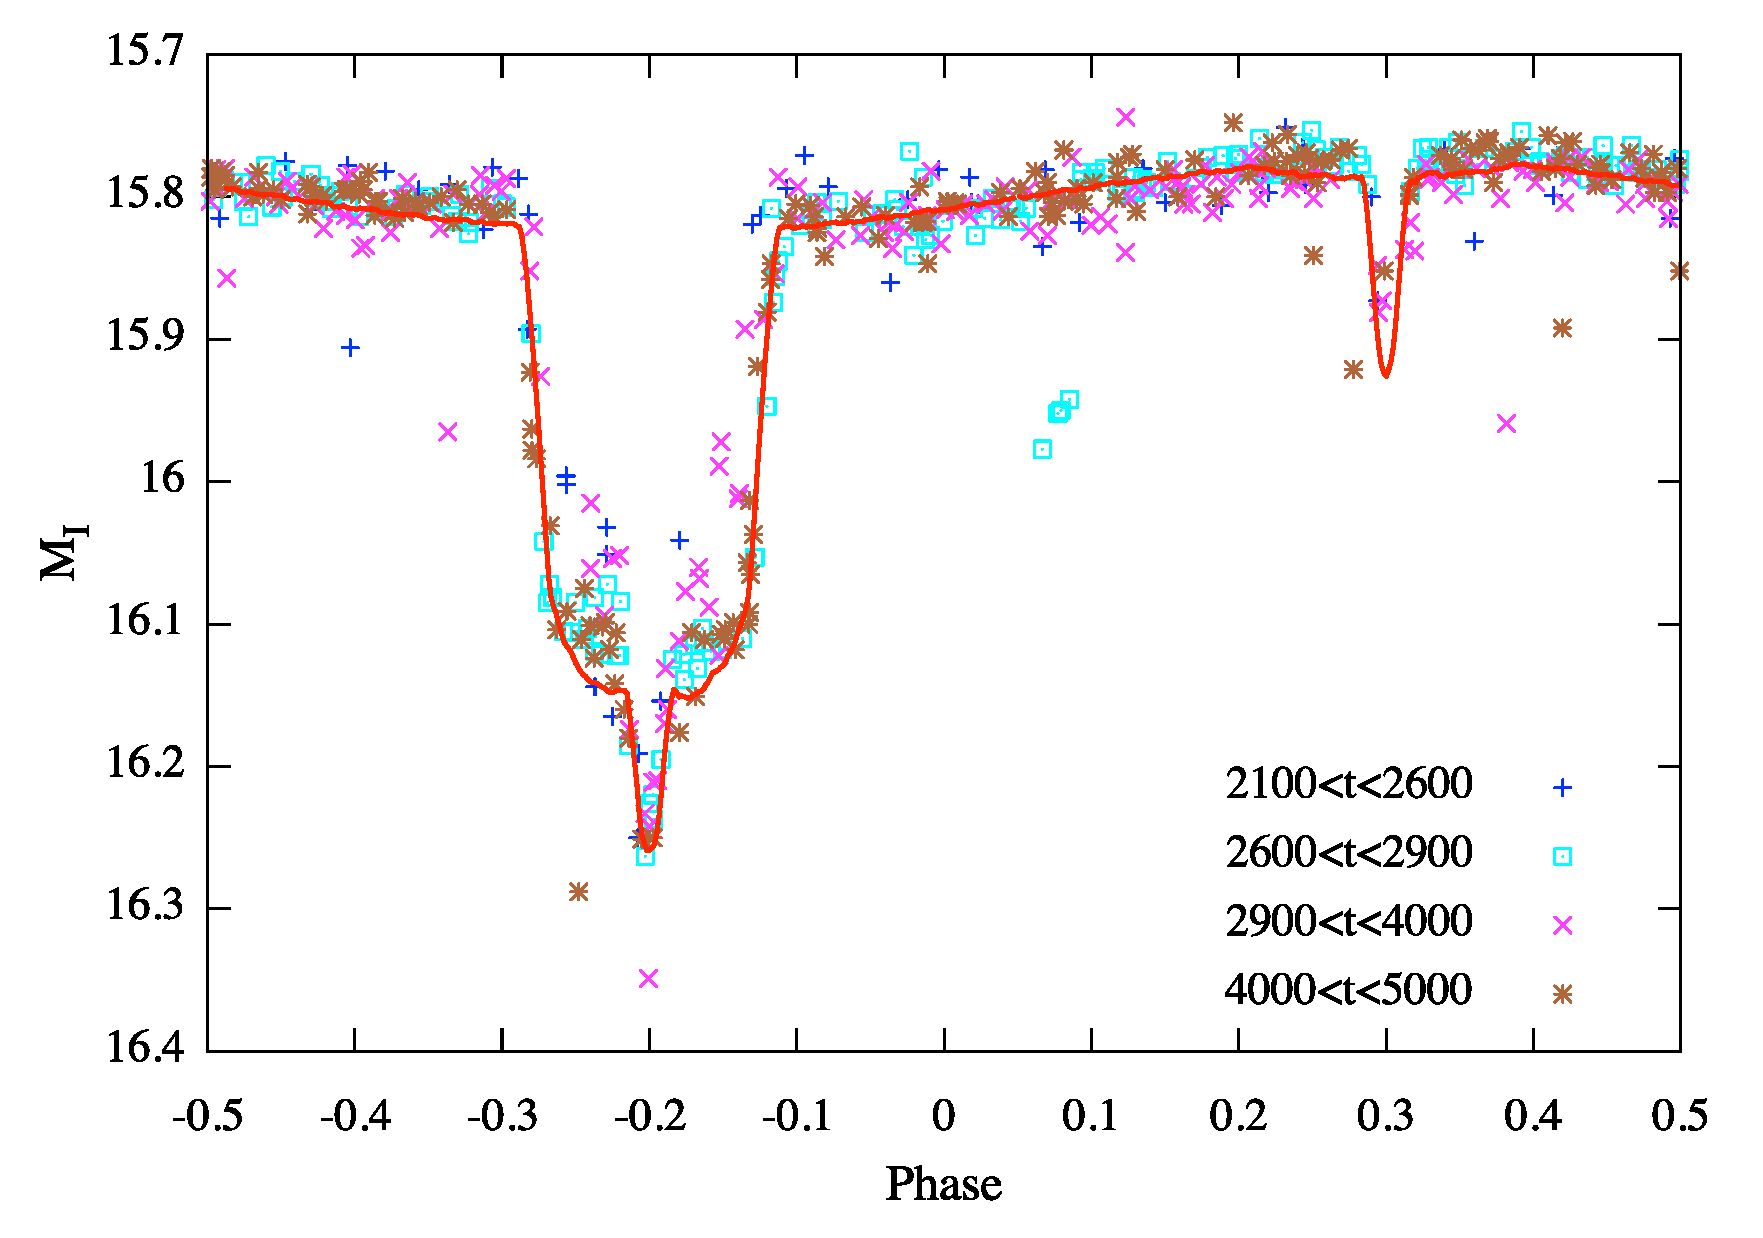
\includegraphics[width=1.0\textwidth]{figures/chapter3/f14_discparam.pdf}
\caption{周期叠加后的 OGLE-III 系统 OGLE-LMC-ECL-17782 以及拟合的光变曲线图。不同点代表不同的时间测得的数据,图中的时间定义为 $t = \tif{HJD} − 245 0000$。关于此  Nightfall  程序的拟合参数请参见表格 \ref{tbl:discparam}。为了显示,我们将此图主掩极大的相位移动了 $\theta_\tif{p}= -0.2$。}
\label{fig:discfit}
\end{figure}

该系统的除了主掩食有浅一些的盘掩食迹象,次掩食也同样可以看到类似的结构,拟合程序 Nightfall 看似并未考虑
次掩时盘对主星的反射,但次掩两侧的长时间浅侧翼也似乎是该反照效应。我们考虑了该系统中正弦相位导致的亮
度变化(振幅大小为 0.025 星等),这正是由于伴星在不同轨道相位上的反射光导致的。同时为了检测该伴星究竟
是否为致密星,我们通过 XMM-Newton 的 LMC 曝光照确认 X-rays 流量为否定的结果。

{\renewcommand{\arraystretch}{1.4}
\begin{table}
\caption{OGLE-LMC-ECL-17782 系统的光变曲线拟合参数}
\label{tbl:discparam}
\centering
\begin{tabularx}{0.9\textwidth}{@{\extracolsep{\fill}}lr}
\hline
Orbital Period & 13.3525 days \\
Primary $T_\tif{eff}$  & 29,000  K  \\
Secondary $T_\tif{eff}$  & 25,500 K   \\
Disk $T_\tif{eff}$  & 6000 K  \\
Primary Roche Fill & 0.176\\
Secondary Roche Fill & 0.158\\
Disk  Roche Fill & 0.97 \\
Orbit Inclination & 87.5$^\circ$ \\
Orbital eccentricity & 0.0 \\
Disk aspect ratio $H/R$  & 0.03 \\
Mass ratio $M_2/M_1$ & 0.8 \\
Primary mass $M_1$     &  $14.3 M_\odot$ \\
Total mass  & $26 M_\odot$ \\
Primary Radius  & $4.6 R_\odot$ \\
Secondary Radius & $3.7 R_\odot$ \\
Disk Radius  & 32.6 $R_\odot$, 0.15 AU \\
Semi-major axis & 70.0 $R_\odot$, 0.33 AU \\
Primary Luminosity & $1.3 \times 10^4 L_\odot $\\ 
Secondary Luminosity & $5000 L_\odot $\\ 
\hline
\end{tabularx}
\medskip \\
对 OGLE-LMC-ECL-17782 系统主星、伴星以及掩食盘的 Nightfall 拟合物理量表格(光变曲线拟合见图 \ref{fig:discfit})。
\end{table}
}

如果该掩食盘在主掩时彻底遮挡住主星,那么通过该掩食深度可以估算得到该盘的光深大概为 $\tau \sim 0.3$。而
部分盘遮挡住主星的情况将会对应更大的光深。通过恒星的总质量(26$\tif{M}_\odot$)我们同样可以估算该盘的
大小为 $\sim 0.15\tif{AU}$。这时考虑到主星的光度($\sim  1.3\times 10^4\,\rm{L_\odot}$),盘吸收了主星 30\% 
的光子能量后,对应于在 0.33 AU 处的温度至少为 $\sim 5500\,\tif{K}$(尚未考虑伴星的辐射)。如果通过盘在整
个掩食周期上所花的时间,则对应与不到 10\% 的遮挡横截面。不管如何,这样的吸收在 Be 恒星周围都很有可能
造成红外超\cite{Waters1988,Dougherty1994}。而温度高达 5500 K 的盘已经完全可以升华所有的盘内固体物质
(即使光变曲线形状更接近于弥散的尘埃盘)。而在如此高的盘遮挡面积下,根据盘的大小以及温度和掩食深度,
不透明度的来源极有可能为 Thompson 散射,以及自由---束缚辐射(如 H\textsc{I} 的光致电离)而不是自由---自由
辐射\cite{Rivinius2013}。而这里我们得到的光变曲线拟合模型并不能很好的限制此系统的性质是因为没有视向曲线
的测量(包括光谱型以及发射谱)。

\subsubsection{OGLE-LMC-ECL-11893} \label{sec:lmc11893}

正如文献 \citen{Scott2014} 中讨论到的,OGLE-LMC-ECL-11893 的光谱显示系统的主星光谱型为 B9III。该系统的
光谱显示主星刚离开主序阶段,也拥有稍稍大于 LMC EB 系统的平均消光。该系统的年龄大约为 150 Myr,消光以
及绝对 V 波段星等,对于光谱型 B9 的恒星而言,该星的绝对光度比主序星阶段常见值明显大一些。虽然该系统双
星的周期为 468 天,但主星的温度非常高,因而星周盘的温度也很可能超过固体升华点。关于该系统的具体讨论以
及掩食盘的详细拟合请参见文献 \citen{Scott2014}。


\section{掩食盘概率估算} \label{sec:discebdiscuz}

与以往 OGLE-II 巡天\cite{Wyrzykowski2003}相比,OGLE-III LMC 巡天的观测时间几乎整整多了一倍,而且归功于
测光精度的提升,OGLE-III LMC 发现的 EBs 数目也比以往多出了一倍。根据文献 \citen{Graczyk2011},LMC EB 
样本星表的完备度几乎达到 90\%(对于 $i$ 波段视星等亮于 18 等的子样本完备度还会更高)。由于 OGLE-III 
LMC 高可信的完备度,我们在这边讨论 LMC EB 样本探测掩食盘的完备度问题。

从文献 \citen{Haisch2001} 中可知,银河系内年轻恒星团的盘出现概率与年龄成反相关性,而且早型恒星盘的寿命
也会明显短过晚型星族,如不足 10\% 的 A-F 型恒星在 3 Myr 年龄内拥有盘,而 T-Tauri 恒星却可高达 30--35\%
\cite{Hernandez2007}。另外年轻恒星是否拥有盘以及盘存活的时间也依赖于恒星的是否处于多星系统中。在对 
1--2 Myr 年龄的 Taurus-Auriga 恒星形成区的搜寻中,Harris 等人发现多星系统的恒星仅有三分之一的比例拥有能
够被探测到星周尘埃盘的毫米波段辐射($\gtrsim$ 10 mJy),与之相比的单星系统却有三分之二的比例
\cite{Harris2012}。考虑到这些因素,我们保守估算在年龄不到 1Myr 的早型星样本中,大概只有 5\% 左右的双星
能够拥有星周盘,而对于 10 Myr 的系统比例则会下降到 1/10。

正是由于这些系统中星周盘存活时标相对较短,因而才会在 LMC 的样本中看到拥有星周盘的双星系统候选体仍处
于主序阶段(当然盘也可能通过后期的质量交换而形成)。在我们分析筛选得到的 2,471 个高信噪比早型 EB 系统
中,至少应该有两个可能的掩食盘候选体(两个通过掩食中平台而发现的盘,如果通过查找 W 型或者不对称型的
掩食内光变曲线还可以找到类似 $\epsilon$ Aur 和 EE Cep 的系统)。如此我们得到的概率 $\gtrsim 1/1000$,应
该和前人在 EBs 中找到盘的比例没有明显的不一致性。然而这里,我们搜索到的两个掩食盘候选体 OGLE-LMC-
ECL-11893 以及 OGLE-LMC-ECL-17782 都应该不是原初恒星盘。可能是由于恒星星风作用\cite{Graczyk2011}或
者快速自转的恒星周围抛射出的喷射盘\cite{Rivinius2013}。相比于 OGLE-LMC-ECL-17782 系统 13.3 天的较短周
期,我们更秦翔宇在距离更远的双星周围找到类似的尘埃盘。

最后需要考虑的是,由于我们探测掩食盘的方法并不能有效的探测  W 型或者不对称型的掩食内光变曲线系统如 $
\epsilon$ Aur 和 EE Cep,因而这边估算的 LMC EB 样本中掩食盘的出现概率还会减少额外的 50\%。通过掩食中
平台的方法来探测 OGLE-LMC-ECL-17782 并不能适用于每个系统 OGLE-LMC-ECL- 11893,因此我们不推荐增加 
\ref{fig:lmcks} 图中的实线方框区域来包括更多的系统,或许更好的做法是利用其他的方法来探测掩食盘可能出现的
特殊形状。



